\section{Въведение}
\subsection{Общо за капилярните мостове}
Капилярните мостове са резултат от минимизирането на повърхността на течност
,,разпъната`` между две твърди тела или течни повърхности с произволна форма.
Това е причината капилярните мостове още да се наричат и ,,капилярни връзки`` (capillary bonds),
тъй като те възникват най-често в практиката като течна връзка при опит за разделяне на две
твърди повърхности омокрени от течност между тях - напр. някои животни могат да ,,залепват`` към
стени, като ,,инжектират`` омокряща течност между \cite{Persson_2007} крайниците си и стената.
Важно значение имат и за агрерирането на частиците в колоидни разтвори, АФМ, омокрянето на прахове и др.
Историята на изследванията им започва с дефинираната от Лагранж задача за мимимизираща повърхност
при дадени граници. Проблемът за намирането на тази повърхност обаче е известен в литературата
като ,,задачата на Плато``, който експерментира със сапунени филми с фиксирани граници.
Той идентифицира седем тела с постоянна гаусова кривина, които описват профила на капилярните мостове:
\begin{enumerate*}
	\item Нодоид с ,,шия``
	\item Катеноид
	\item Ундулоид с ,,шия``
	\item Цилиндър
	\item Ундулоид с ,,гърбица``
	\item Сфера
	\item Нодоид с ,,гърбица``.
\end{enumerate*}
За 1. до 5. капилярните сили трябва да са на привличане, за сфера да са 0, а за 7. да са на
отблъскване. При \cite{Kralchevsky}
Когато границите са тороидни (,,кръгли``), то при сапунените филми се получава профил на катеноид \autoref{fig:soap_cath}.
\begin{figure}[h]
	\centering
	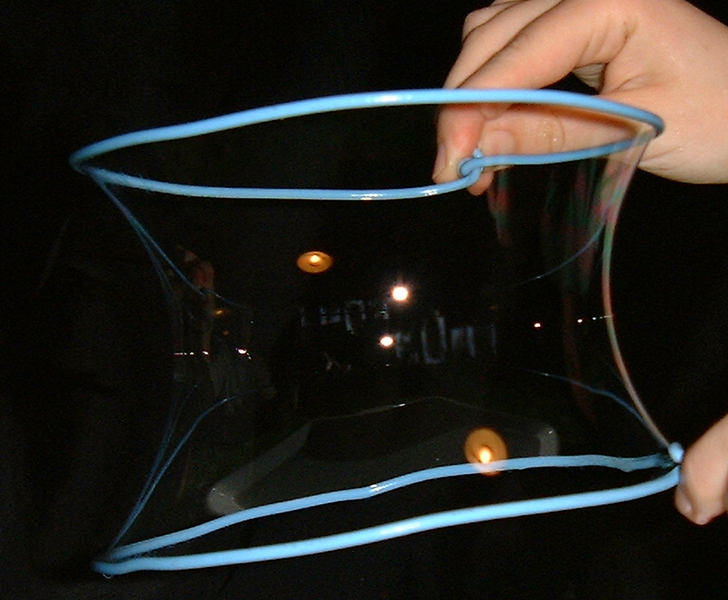
\includegraphics[width=0.4\linewidth]{cathenoid_soap.png}
	\caption{Сапунен филм с тороидни граници (телчетата).\cite{Soap_cathenoid}}
	\label{fig:soap_cath}
\end{figure}
\subsection{Експериментални основи}
Най-простите (геометрично) повърхности, между които може да се формира капилярен мост са две плоски пластини.
\textit{Иван Т. Иванов} \cite{ivan_phd} изследва динамиката и статиката на такива капилярни мостове.
На \autoref{fig:cups_full} са представени кадри от заснето с високоскоростта камера късане на моста.
Вижда се, че по време на целия процес - от равновесното състояние до момента на пълно скъсване, можем
да разделим геометрично моста грубо на два мениска и талия. Двата мениска служат като резервоари, към които
течността ,,напуска`` от талията. 
\begin{figure*}[h]
	\centering
	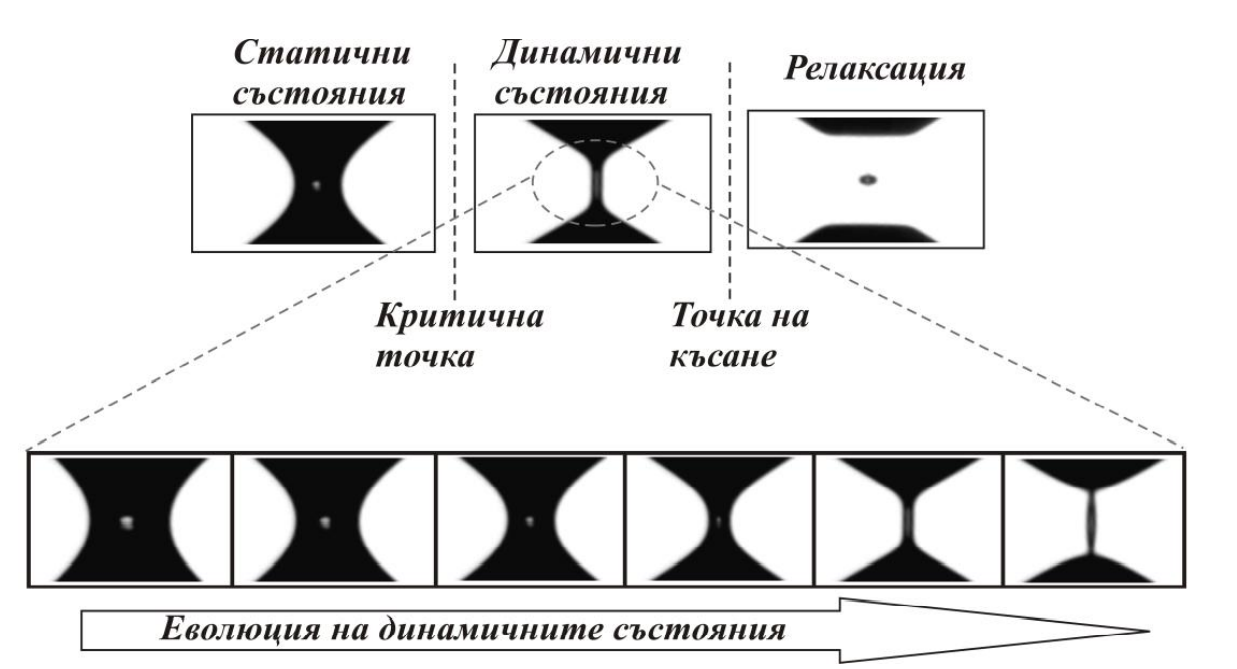
\includegraphics[width=0.7\linewidth]{chashski_full.png}
	\caption{Късане на капилярен мост формиран между две пластини \cite{ivan_phd}}
	\label{fig:cups_full}
\end{figure*}
Още повече: всяка от по-сложните геометрии представени по-горе, може да бъде апроксимирана с цилиндър.
Разбира се всяко такова драстично опростяване на една геометрия трябва да се прави изключително внимателно,
тъй като във всеки модел трябва да има баланс - да е достатъчно прост, за да позволява аналитично разглеждане,
но и да е достатъчно подробен, за да са полезни на практика следствията от него.
Цилиндърът има постоянна средна кривина, тъй като $H(\vec{x}) = 1/r_{c} = const$, където $\vec{x}$ e 
радиус-вектор на тримерна точка от повърхността на цилиндъра. Това по същество представлява една линеаризация
на задачата.
В настоящия труд освен \cite{ivan_phd}, не са провеждани експерименти, които да имат насочената цел да проверят
получените модели. Въпреки това както ще стане ясно по-нататък, са направени някои оценки и интерпретации на база
литературни данни за различни параметри.